\subsection{Quantitative Evaluation of Segmentation Performance}

Table~\ref{tab:loss_comparison_small_lesion} summarizes the 5-fold
cross-validation results for all loss functions under the same
\texttt{nnUNet} training and evaluation pipeline. Since the architecture,
preprocessing, and evaluation protocol are fixed, the differences mainly
reflect the effect of the training objective. Overall, nnUNet-CATMIL
provides the strongest balance between voxel-level segmentation accuracy,
boundary quality, and missed-lesion reduction.

For global segmentation performance, nnUNet-CATMIL obtains the highest
Dice score of 0.7834, compared with 0.7796 for nnUNet-DiceCE, 0.7706 for
nnUNet-Tversky, and 0.7802 for nnUNet-FocalTversky. The Dice improvement
is moderate, but it is accompanied by a clearer improvement in boundary
accuracy. In particular, nnUNet-CATMIL achieves the lowest HD95
(7.9817 mm), improving over nnUNet-DiceCE (9.0372 mm), nnUNet-Tversky
(10.2408 mm), and nnUNet-FocalTversky (8.2060 mm). This suggests that
the proposed loss does not only improve overlap, but also reduces large
boundary deviations.

\begin{center}
\captionof{table}{Comparison of the proposed CATMIL loss with standard loss functions for small-lesion segmentation. Best values are shown in \textbf{bold}, and second-best values are \underline{underlined}. Higher is better for Dice, Lesion F1, and Small Lesion Recall, while lower is better for HD95, FN metrics, and FP Volume.}
\label{tab:loss_comparison_small_lesion}
\resizebox{\textwidth}{!}{%
\begin{tabular}{lcccc}
\toprule
\textbf{Metric} & \textbf{nnUNet-CATMIL (ours)} & \textbf{nnUNet-DiceCE} & \textbf{nnUNet-Tversky} & \textbf{nnUNet-FocalTversky} \\
\midrule
Dice $\uparrow$ 
& \textbf{0.7834} & 0.7796 & 0.7706 & \underline{0.7802} \\

HD95 (mm) $\downarrow$ 
& \textbf{7.9817} & 9.0372 & 10.2408 & \underline{8.2060} \\

Small Lesion Recall $\uparrow$ 
& \textbf{0.8730} & 0.7956 & \underline{0.8336} & 0.8313 \\

Lesion F1 $\uparrow$ 
& 0.7571 & \underline{0.8433} & 0.8402 & \textbf{0.8455} \\

FN Count $\downarrow$ 
& \textbf{2.5667} & 4.9500 & 3.7667 & \underline{3.7000} \\

FN Volume Fraction $\downarrow$ 
& \textbf{0.0214} & 0.0341 & 0.0257 & \underline{0.0250} \\

FP Volume (mm$^3$) $\downarrow$ 
& \textbf{1537} & 1819 & 2621 & 2282 \\
\bottomrule
\end{tabular}%
}
\end{center}

The main advantage of nnUNet-CATMIL is observed in lesion sensitivity.
It achieves the highest Small Lesion Recall (0.8730), outperforming
nnUNet-DiceCE by 7.74 percentage points and also exceeding both
nnUNet-Tversky (0.8336) and nnUNet-FocalTversky (0.8313). This gain is
also reflected in the false-negative metrics. nnUNet-CATMIL reduces the
mean FN Count to 2.5667, whereas nnUNet-DiceCE misses 4.9500 lesions on
average. Similarly, the FN Volume Fraction decreases to 0.0214, compared
with 0.0341 for nnUNet-DiceCE and approximately 0.025 for the
Tversky-based losses. These results indicate that the proposed objective
is particularly effective in reducing complete lesion misses.

This improvement in sensitivity does not correspond to a large increase
in false-positive volume. nnUNet-CATMIL produces the lowest FP Volume
(1537 mm$^3$), compared with 1819 mm$^3$ for nnUNet-DiceCE,
2621 mm$^3$ for nnUNet-Tversky, and 2282 mm$^3$ for
nnUNet-FocalTversky. Therefore, the proposed loss improves lesion
detection while keeping the total volume of false-positive voxels low.
However, nnUNet-CATMIL has a lower Lesion F1 score (0.7571) than
nnUNet-DiceCE (0.8433) and nnUNet-FocalTversky (0.8455). This indicates
a lesion-level precision trade-off, likely caused by additional small
connected components or fragmented predictions. In contrast,
nnUNet-FocalTversky achieves the best Lesion F1, but it does not provide
the same level of small-lesion recall or FN reduction as nnUNet-CATMIL.

Among the baseline losses, nnUNet-DiceCE remains competitive in Dice and
Lesion F1, but it shows the weakest performance in missed-lesion metrics.
nnUNet-Tversky reduces FN Count relative to nnUNet-DiceCE, but this comes
with lower Dice and worse HD95, indicating less stable segmentation
boundaries. nnUNet-FocalTversky improves lesion-level balance and
boundary accuracy compared with nnUNet-Tversky, but still remains below
nnUNet-CATMIL in small-lesion recall and false-negative reduction.


\subsection{Analysis of Missed Lesion Errors Across Sizes}

To further examine missed-lesion behavior, we analyze lesion-level false
negative metrics in addition to voxel-level overlap scores.
Figure~\ref{fig:fn_baseline} shows that nnUNet-CATMIL produces the lowest
number of missed lesions among all compared methods. The mean FN lesion
count decreases to 2.57 with nnUNet-CATMIL, compared with 3.70 for
nnUNet-FocalTversky, 3.77 for nnUNet-Tversky, and 4.95 for
nnUNet-DiceCE. The difference is especially clear relative to
nnUNet-DiceCE, which misses nearly twice as many lesions.

The same trend is observed for the miss rate. nnUNet-CATMIL achieves the
lowest miss rate (0.092), while nnUNet-Tversky and nnUNet-FocalTversky
remain at approximately 0.120, and nnUNet-DiceCE reaches 0.153. The
agreement between FN count and miss rate indicates that the reduction in
missed lesions is not an artifact of a single metric. Instead, the
proposed loss consistently shifts the prediction behavior toward lesion
presence detection.

This behavior is important for small-lesion segmentation. In sparse
lesion settings, a model may obtain a reasonable Dice score while still
missing several small components completely. nnUNet-CATMIL reduces this
failure mode by encouraging the model to detect lesions that standard
losses tend to overlook. As a result, its errors are less dominated by
complete lesion misses, even when some predicted regions are not perfectly
delineated.

\begin{figure}[htbp]
    \centering
    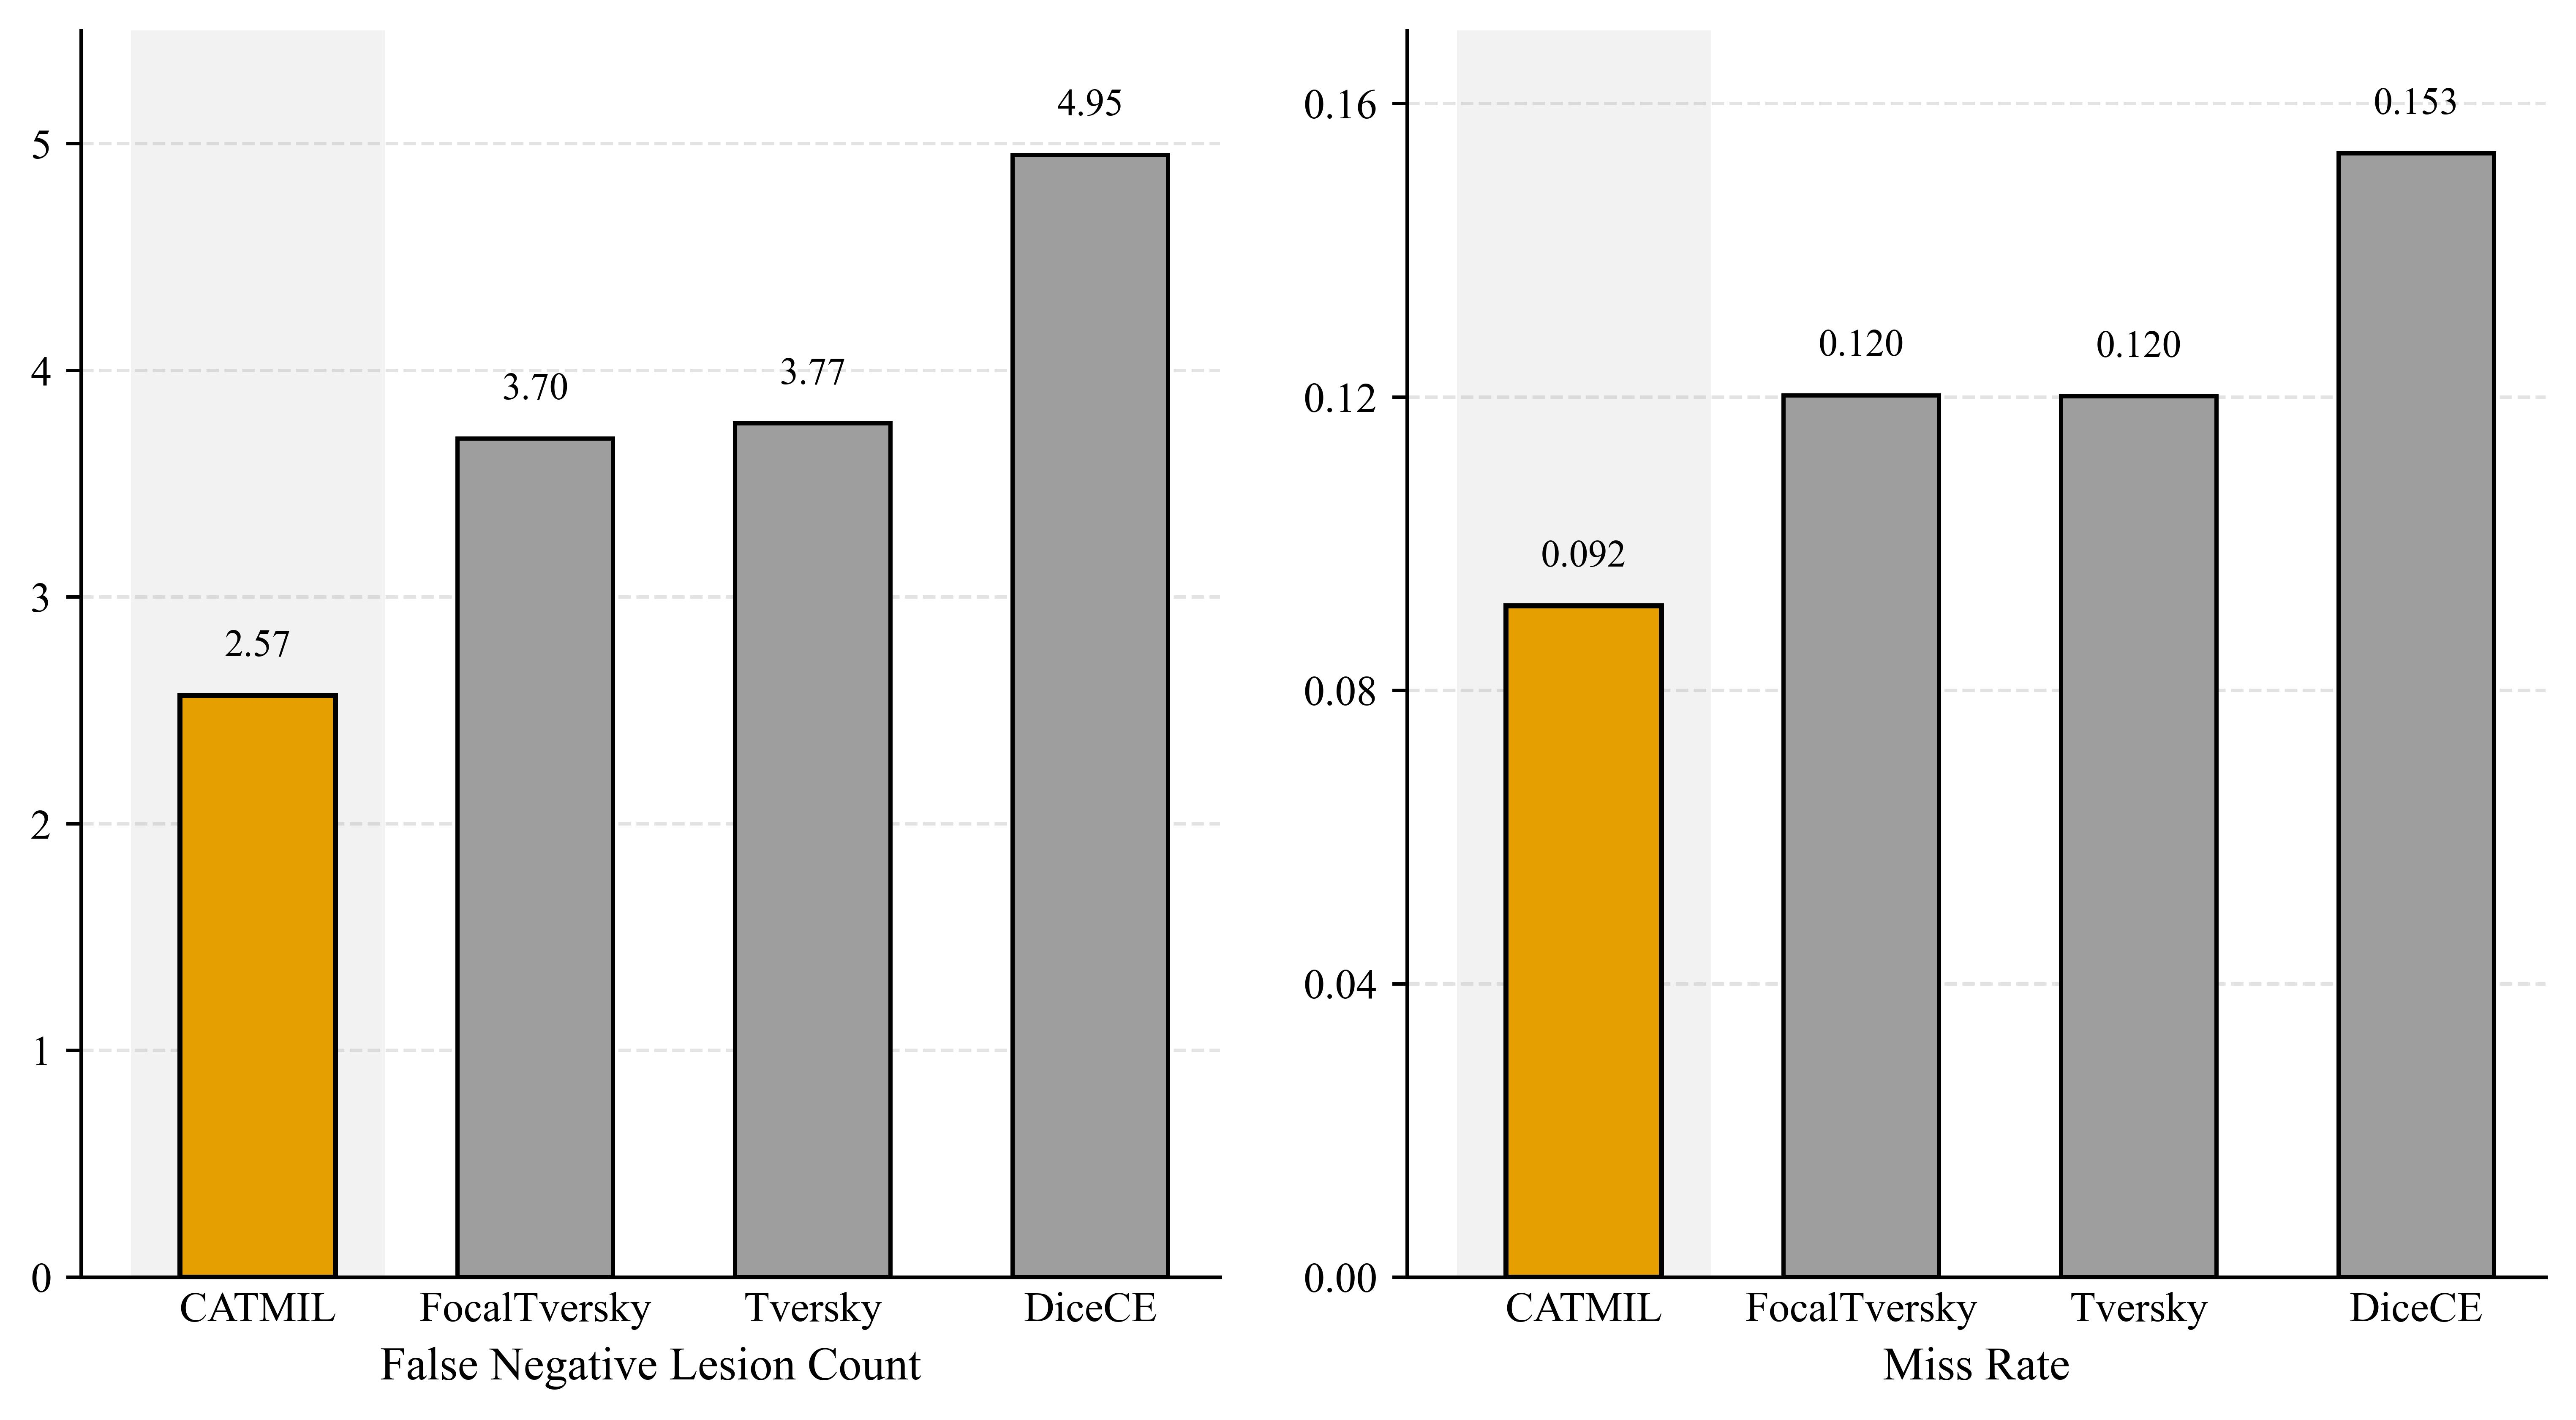
\includegraphics[width=\textwidth]{figures/fn_step1_combined.jpeg}
    \caption{Baseline false negative (FN) analysis across models using lesion-level metrics. From left to right: FN lesion count, lesion recall, and miss rate. nnUNet-CATMIL is highlighted with diagonal stripes.}
    \label{fig:fn_baseline}
\end{figure}

The global FN analysis shows that nnUNet-CATMIL misses fewer lesions
overall, but it does not specify whether the improvement is concentrated
in a particular lesion-size range. We therefore evaluate lesion recall
across size groups in Figure~\ref{fig:fn_recall_by_size}.

nnUNet-CATMIL achieves the highest recall across all lesion-size groups.
The largest relative improvement appears for the smallest lesions
($\leq$10 voxels), where recall increases from 0.14 with nnUNet-DiceCE to
0.33 with nnUNet-CATMIL. This indicates that many tiny lesions that are
completely missed by the standard DiceCE objective can be recovered by the
proposed loss.

The improvement also extends to larger but still small lesions. For
lesions $\leq$50 voxels, nnUNet-CATMIL reaches a recall of 0.79, compared
with 0.71 for nnUNet-DiceCE. For medium-sized lesions ($\leq$200 voxels),
nnUNet-CATMIL achieves 0.95 recall, again outperforming the baselines.
For large lesions ($>200$ voxels), where all methods already perform
well, nnUNet-CATMIL reaches a recall of 1.00. Therefore, the proposed
loss improves detection of the most difficult small lesions without
reducing performance on larger lesions.

These findings suggest that nnUNet-CATMIL reduces the size-dependent bias
commonly observed in lesion segmentation. Standard losses tend to favor
larger and easier structures, whereas CATMIL improves the low-volume
lesion regime while preserving detection of larger components. This
produces a more balanced lesion detection profile across scales.

\begin{figure}[htbp]
    \centering
    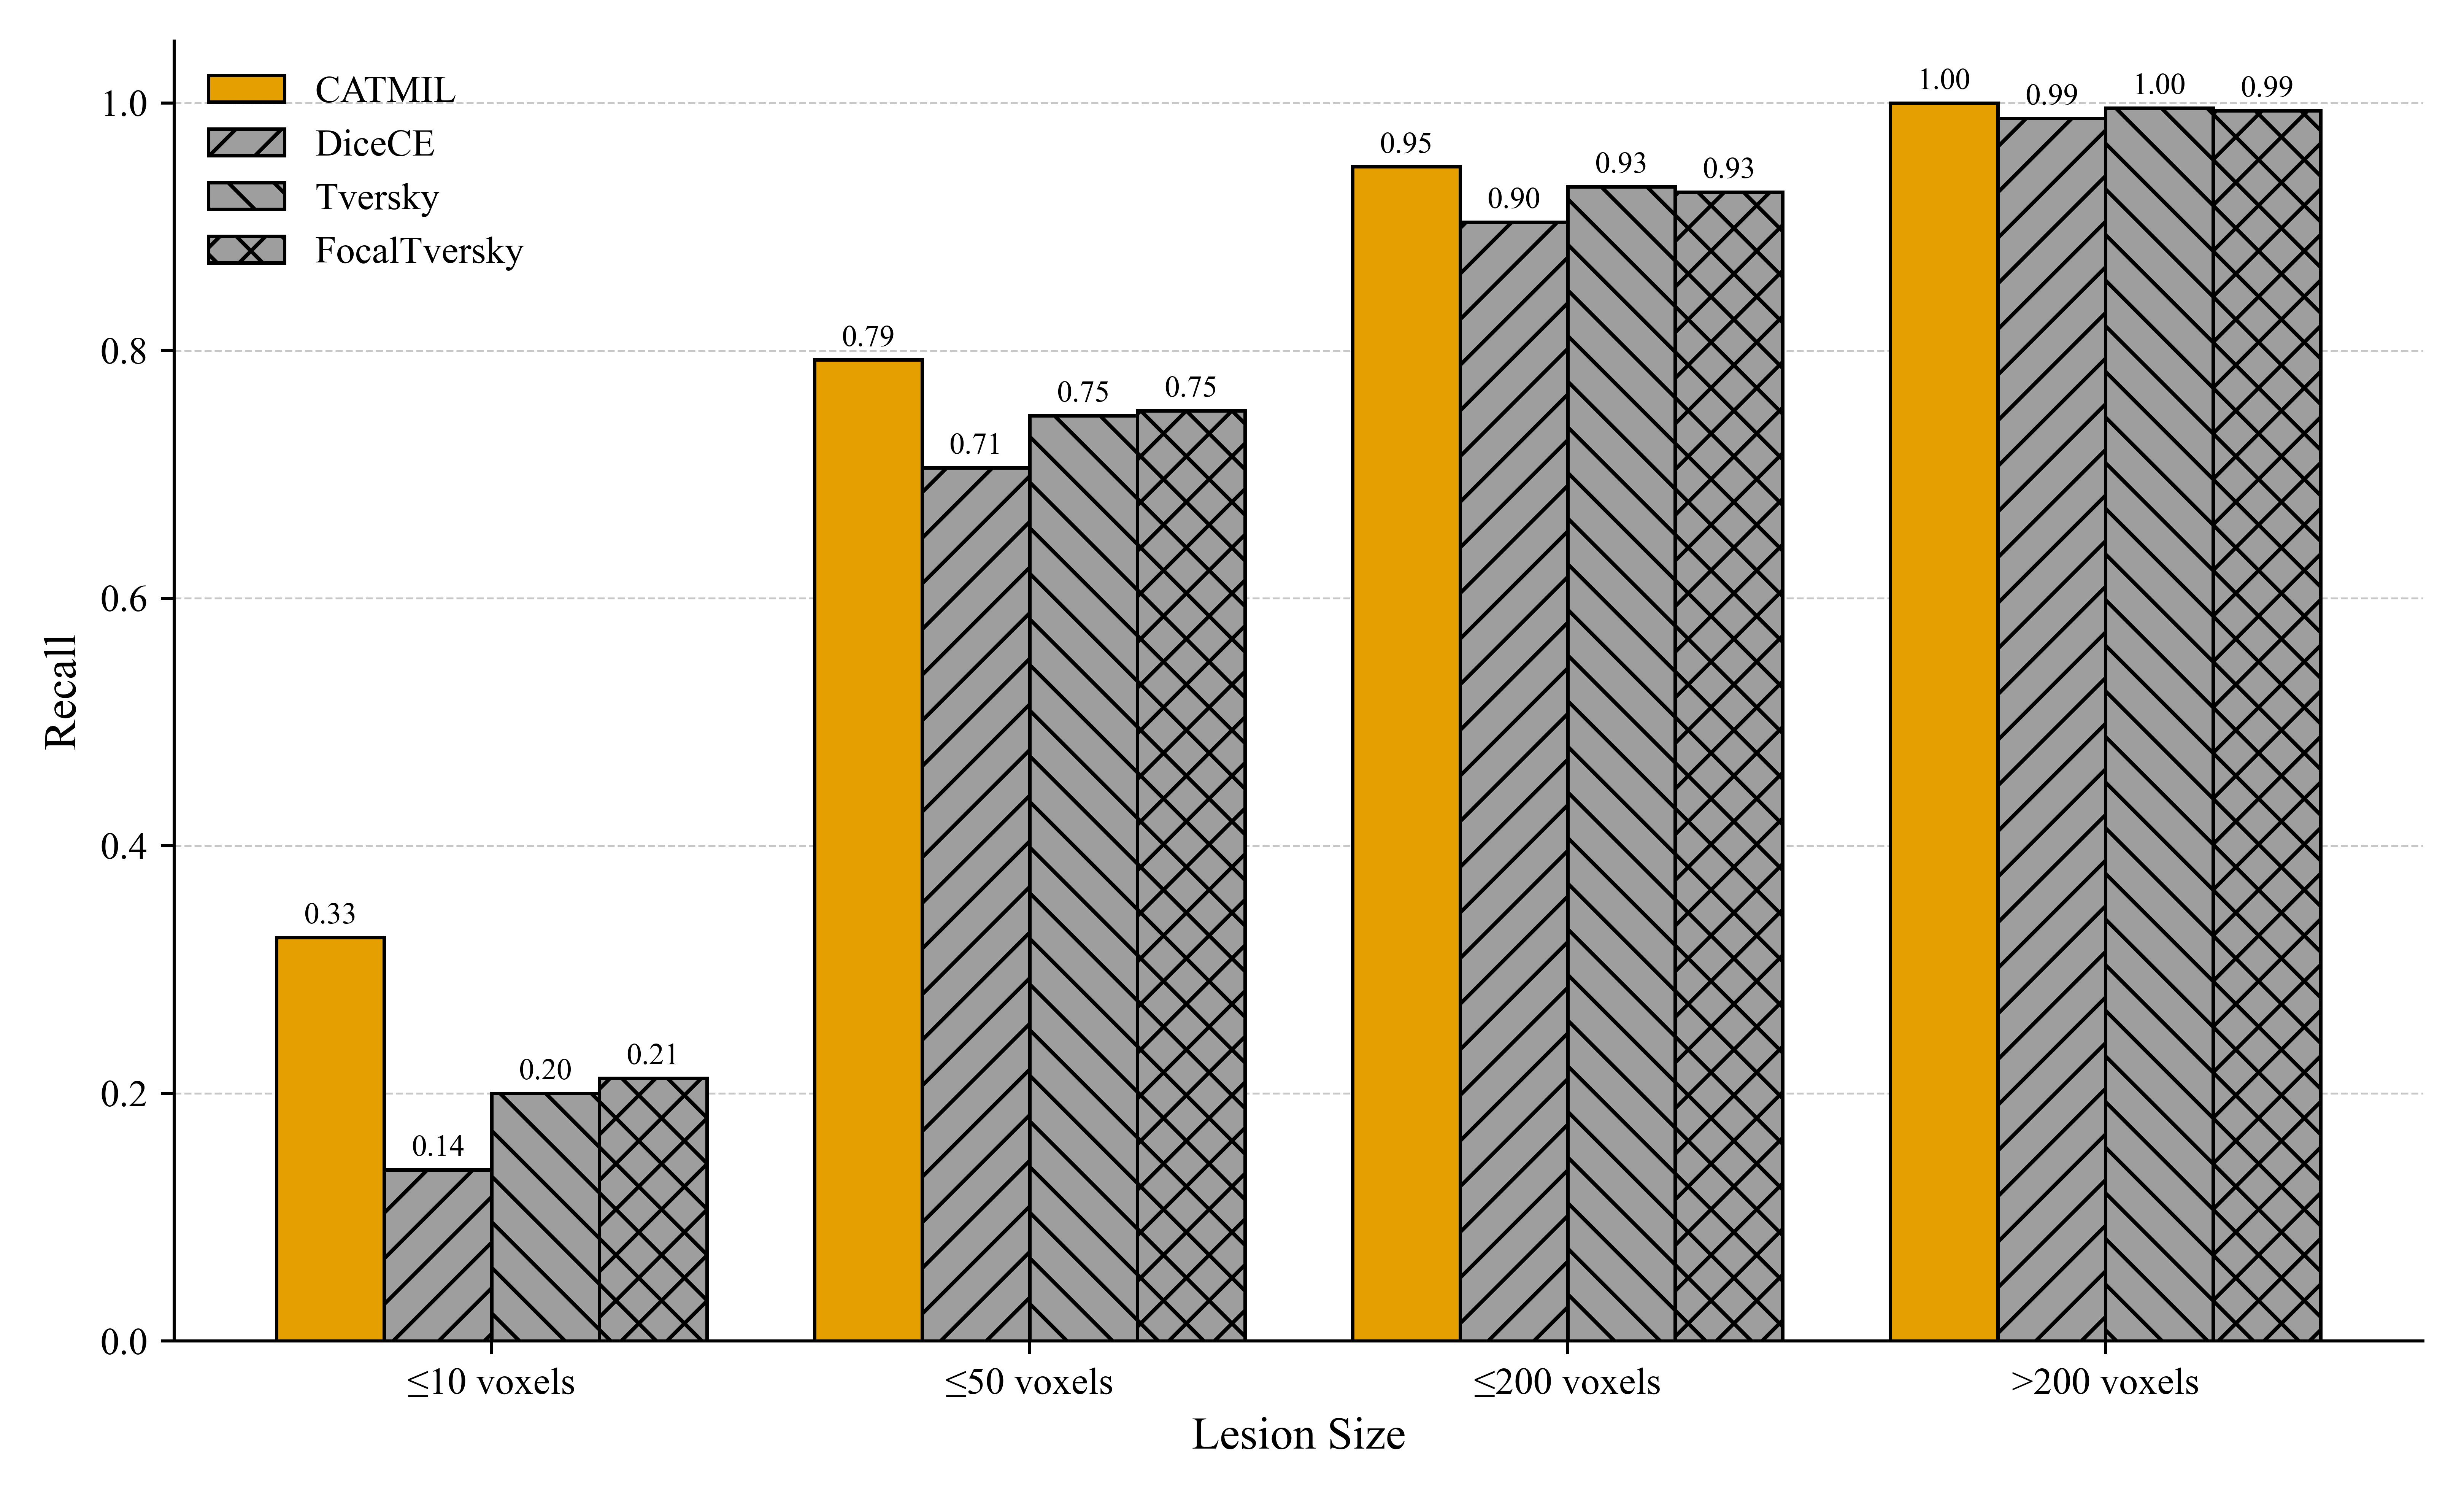
\includegraphics[width=\textwidth]{figures/fn_recall_by_size.jpeg}
    \caption{Recall by lesion size in voxels for different loss functions. Higher recall indicates fewer false negatives.}
    \label{fig:fn_recall_by_size}
\end{figure}


\subsection{Case-Based Qualitative Analysis of Lesion Segmentation}

\begin{figure}[t]
    \centering
    \includegraphics[width=\linewidth]{figures/P47_T1_fold1_slice94_segmentation_comparison.jpeg}
    \caption{
    Segmentation comparison for Case P47\_T1.
    Green indicates correctly detected lesion voxels, red indicates missed
    regions (false negatives), and yellow indicates false positives.
    }
    \label{fig:case_p47}
\end{figure}

Figure~\ref{fig:case_p47} shows Case P47\_T1, where lesions appear in a
clustered pattern with moderate size and relatively visible contrast. The
lesions include components of approximately 20--50 voxels, and their
contrast relative to the surrounding tissue is sufficiently high
(LCNR $>$ 1.5) to make them detectable, although their limited size still
poses a segmentation challenge. All models detect the larger components,
but nnUNet-DiceCE and nnUNet-Tversky miss several smaller regions.
nnUNet-CATMIL detects more of these small components and produces a more
spatially consistent prediction. The segmented regions also align more
closely with the ground truth, suggesting improved handling of clustered
small-lesion structures.

\begin{figure}[t]
    \centering
    \includegraphics[width=\linewidth]{figures/P49_T2_fold1_slice90_segmentation_comparison.jpeg}
    \caption{
    Segmentation comparison for Case P49\_T2.
    Green indicates correctly detected lesion voxels, red indicates missed
    regions (false negatives), and yellow indicates false positives.
    }
    \label{fig:case_p49}
\end{figure}

Case P49\_T2, shown in Figure~\ref{fig:case_p49}, contains elongated
lesions with heterogeneous intensity and less distinct boundaries. The
lesion contrast is relatively low (LCNR $\sim$0.8--1.2), and the weaker
boundary sharpness makes localization more ambiguous. Under this setting,
baseline losses show several missed regions, particularly for small and
low-contrast components, and they also introduce scattered false-positive
areas. nnUNet-FocalTversky improves lesion recovery but produces
irregular segmentation boundaries. nnUNet-CATMIL provides a more balanced
prediction by detecting a larger portion of the difficult lesions while
maintaining more coherent segmentation regions. Although some small false
positives remain, they are limited and do not dominate the predicted mask.

\begin{figure}[t]
    \centering
    \includegraphics[width=\linewidth]{figures/P52_T2_fold0_slice87_segmentation_comparison.jpeg}
    \caption{
    Segmentation comparison for Case P52\_T2.
    Green indicates correctly detected lesion voxels, red indicates missed
    regions (false negatives), and yellow indicates false positives.
    }
    \label{fig:case_p52}
\end{figure}

Figure~\ref{fig:case_p52} presents Case P52\_T2, which represents a highly
sparse lesion scenario. The lesions are very small, with volumes below
approximately 10 voxels, and their contrast is close to the background
noise level (LCNR $\approx$1.0). Such cases are sensitive to minor
prediction errors because the target structures occupy only a few voxels.
Most models detect the main lesion regions, but nnUNet-CATMIL also
produces a small isolated false-positive blob. This example illustrates
the sensitivity-oriented behavior of CATMIL: the model is less likely to
miss weak lesion signals, but this can occasionally introduce small
spurious components in extremely sparse cases. Nevertheless, the main
lesion locations remain correctly identified.

Across the three cases, lesion difficulty is determined by more than
volume alone. Low contrast, weak boundaries, elongated shapes, and sparse
spatial distribution all increase the risk of missed detections. The
qualitative results are consistent with the quantitative findings:
nnUNet-CATMIL improves recovery of subtle lesions and preserves coherent
lesion structures, while the additional false positives are generally
small and localized.


\subsection{Analysis of False Positives and Post-Processing}

The results in Table~\ref{tab:loss_comparison_small_lesion} show an
apparent trade-off in nnUNet-CATMIL. The model achieves the best Dice,
HD95, Small Lesion Recall, FN Count, FN Volume Fraction, and FP Volume,
but its Lesion F1 is lower than the baselines. To interpret this behavior,
we further examine the nature of its false positives.

nnUNet-CATMIL reaches high lesion-level recall, but its lesion-level
precision is lower. This means that the model detects most true lesions,
but it also predicts additional connected components. However, the low FP
Volume indicates that these additional components are not large
over-segmented regions. Instead, the model predicts many small components:
the average number of predicted connected components is much higher than
the number of ground-truth lesions, while the total false-positive volume
remains the lowest among all methods. This suggests that the lower Lesion
F1 is mainly caused by small fragmented predictions rather than extensive
false-positive regions.

The spatial distribution of false positives supports this interpretation.
Most false-positive voxels are located close to ground-truth lesions, with
a near-voxel fraction of approximately 0.7--0.8 and a median distance of
only 1--2 mm. Therefore, many false positives correspond to small
near-lesion fragments or boundary-adjacent predictions, rather than
distant isolated errors. This error pattern is consistent with a model
that is more sensitive to weak lesion evidence.

Since many of these components are small, we apply a simple
post-processing step that removes connected components smaller than
5 voxels. The same procedure is applied to all models, and the resulting
metrics are reported in
Table~\ref{tab:loss_comparison_small_lesion_pp5}.

\begin{center}
\captionof{table}{Comparison of models after post-processing with minimum connected-component size of 5 voxels.}
\label{tab:loss_comparison_small_lesion_pp5}
\resizebox{\textwidth}{!}{%
\begin{tabular}{lcccc}
\toprule
\textbf{Metric} & \textbf{nnUNet-CATMIL (ours)} & \textbf{nnUNet-DiceCE} & \textbf{nnUNet-Tversky} & \textbf{nnUNet-FocalTversky} \\
\midrule
Dice $\uparrow$ 
& \textbf{0.7842} & 0.7797 & 0.7707 & \underline{0.7803} \\

HD95 (mm) $\downarrow$ 
& \textbf{8.1028} & 9.0895 & 10.3585 & \underline{8.2297} \\

Small Lesion Recall $\uparrow$ 
& \textbf{0.8554} & 0.7853 & \underline{0.8223} & 0.8196 \\

Lesion F1 $\uparrow$ 
& 0.8415 & \textbf{0.8586} & 0.8532 & \underline{0.8582} \\

FN Count $\downarrow$ 
& \textbf{3.1333} & 5.2333 & \underline{4.0667} & 4.0833 \\

FN Volume Fraction $\downarrow$ 
& \textbf{0.0238} & 0.0353 & 0.0277 & \underline{0.0270} \\

FP Volume (mm$^3$) $\downarrow$ 
& \textbf{1515} & \underline{1815} & 2618 & 2279 \\
\bottomrule
\end{tabular}%
}
\end{center}

Post-processing produces a similar effect across all losses. Removing
very small connected components slightly reduces recall-related metrics
and increases FN-related metrics, while improving Lesion F1. This
expected trend confirms that the filtering step removes small predicted
regions, some of which correspond to false positives and some of which may
overlap with true small lesions.

For nnUNet-CATMIL, the effect is particularly informative. Lesion F1
increases substantially from 0.7571 before post-processing to 0.8415
after filtering, showing that many of the lesion-level precision errors
come from very small components. At the same time, nnUNet-CATMIL retains
the best Dice score, the lowest HD95, the highest Small Lesion Recall,
the lowest FN Count, the lowest FN Volume Fraction, and the lowest FP
Volume after post-processing. Therefore, the post-processed results
preserve the main advantage of CATMIL while reducing the lesion-level
precision penalty.

Overall, these results indicate that nnUNet-CATMIL favors sensitivity to
small and weak lesion signals. This sensitivity can introduce additional
small connected components, but these components are limited in volume and
can be reduced by a simple model-agnostic post-processing step. After
filtering, CATMIL continues to show the strongest overall balance between
segmentation quality, missed-lesion reduction, and false-positive control.